% SC4021 Chapter 2: Boolean vs Vector Space
\chapter{Boolean Retrieval vs.\ Vector Space Model}\label{ch:boolean-vector}
\begin{center}\small\textit{From exact set operations to geometric ranking: why ``contains the word'' is not enough and how angles between vectors give order.}\end{center}

\noindent\fbox{\parbox{\dimexpr\linewidth-2\fboxsep-2\fboxrule}{%
\textbf{From zero: no retrieval model assumed.} We start from sets (SC1007 review), build Boolean retrieval as set intersection/union, expose its brittle ranking, then place every document as a point in term-space and rank by cosine.}}
\vspace{0.4em}

\section*{Learning Outcomes}
After this chapter you will be able to:
\begin{enumerate}[label=(L\arabic*)]
  \item execute Boolean queries via postings sets and explain their limits;
  \item represent documents/queries as term vectors and build the term-document matrix;
  \item compute cosine similarity and rank documents for a query;
  \item compare Boolean vs.\ ranked retrieval and choose per task;
  \item handle phrase and wildcard intuition via positional sets.
\end{enumerate}

% ============================================================
\section{Boolean Retrieval: Terms as Sets}\label{sec:boolean}
\paragraph{Intuition.} If the query is \texttt{cats AND dogs}, a document qualifies iff its term set contains both words -- a set intersection. \texttt{OR} is union, \texttt{NOT} is complement. Simple and exact, but you either match or you do not; there is no ``best'' among the matches, and one missing synonym kills recall.

\paragraph{Formal model.} For term $t$, let $P(t)=\{d\in\mathcal{C}: t\in d\}$ be its \emph{postings set}. Then
\begin{equation}
P(t_1 \text{ AND } t_2)=P(t_1)\cap P(t_2),\quad
P(t_1 \text{ OR } t_2)=P(t_1)\cup P(t_2),\quad
P(\text{NOT } t)=\mathcal{C}\setminus P(t).
\end{equation}
With an inverted index (Ch.~4), $P(t)$ is stored sorted; intersection is a linear merge $O(|P(t_1)|+|P(t_2)|)$ or faster with skips.

\begin{definition}[Boolean Retrieval]
Given query $q$ in disjunctive/conjunctive normal form over terms, $Answer(q)$ is defined recursively via the set equations above. Result is an \emph{unordered} set; no ranking.
\end{definition}

\begin{figure}[h]\centering
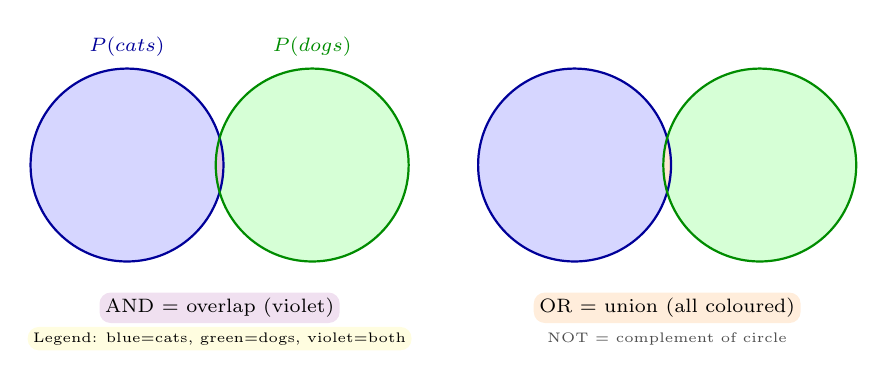
\begin{tikzpicture}[font=\scriptsize, scale=0.98]
  % Venn for AND/OR
  \begin{scope}
    \fill[blue!16] (-1.2,0) circle (1.25cm);
    \fill[green!16] (1.2,0) circle (1.25cm);
    \begin{scope}
      \clip (-1.2,0) circle (1.25cm);
      \fill[violet!22] (1.2,0) circle (1.25cm);
    \end{scope}
    \draw[thick, blue!60!black] (-1.2,0) circle (1.25cm) node[above, yshift=1.25cm] {$P(\text{cats})$};
    \draw[thick, green!55!black] (1.2,0) circle (1.25cm) node[above, yshift=1.25cm] {$P(\text{dogs})$};
    \node[fill=violet!12, rounded corners, inner sep=2pt] at (0,-1.85) {AND = overlap (violet)};
    \node[font=\tiny, fill=yellow!12, rounded corners, inner sep=2pt] at (0,-2.25) {Legend: blue=cats, green=dogs, violet=both};
  \end{scope}
  \begin{scope}[xshift=5.8cm]
    \fill[blue!16] (-1.2,0) circle (1.25cm);
    \fill[green!16] (1.2,0) circle (1.25cm);
    \begin{scope}
      \clip (-1.2,0) circle (1.25cm);
      \clip (1.2,0) circle (1.25cm);
      \fill[orange!18] (-1.2,0) circle (1.25cm);
    \end{scope}
    \fill[blue!16] (-1.9,0) -- (-1.2,1.25) arc (90:270:1.25) -- cycle;
    \fill[green!16] (1.9,0) -- (1.2,1.25) arc (90:-90:1.25) -- cycle;
    \draw[thick, blue!60!black] (-1.2,0) circle (1.25cm);
    \draw[thick, green!55!black] (1.2,0) circle (1.25cm);
    \node[fill=orange!14, rounded corners, inner sep=2pt] at (0,-1.85) {OR = union (all coloured)};
    \node[font=\tiny, text=gray!60!black] at (0,-2.25) {NOT = complement of circle};
  \end{scope}
\end{tikzpicture}
\caption{Boolean operations as set operations: AND is intersection, OR is union.}
\label{fig:boolean-venn}
\end{figure}

\begin{example}[Boolean evaluation]
\begin{sloppypar}
Collection: $d_1$=\{cats,dogs\}, $d_2$=\{cats\}, $d_3$=\{dogs,birds\}, $d_4$=\{cats,dogs,birds\}. Then $P(\text{cats})=\{1,2,4\}$, $P(\text{dogs})=\{1,3,4\}$. Query \texttt{cats AND dogs}: $\{1,2,4\}\cap\{1,3,4\}=\{1,4\}$ (unordered).\\ Query \texttt{cats AND NOT dogs}: $\{1,2,4\}\setminus\{1,3,4\}=\{2\}$.
\end{sloppypar}
\end{example}

Limits: no ranking among $\{1,4\}$, synonym failure (\texttt{feline} $\neq$ \texttt{cats}), and verbose queries to express ``more cats than dogs matters.''

% ============================================================
\section{Vector Space: Documents as Vectors}\label{sec:vector}
\paragraph{Intuition.} Place every term as an axis in a $V$-dimensional space. Document $d$ becomes a vector $\vec{d}\in\mathbb{R}^V$ where coordinate $t$ is the weight of term $t$ in $d$ (for now, $0/1$ or count). Query $\vec{q}$ is another vector. Documents that point in a similar direction as the query are more relevant -- measured by the angle between them.

\paragraph{Formal.} Let vocabulary $\mathcal{V}=\{t_1,\dots,t_V\}$. Define term-document matrix $M\in\mathbb{R}^{V\times N}$ with $M_{t,d}=w(t,d)$ (weight). Column $M_{\cdot,d}=\vec{d}$ is a doc vector; query vector $\vec{q}$ has $q_t=w(t,q)$. For now $w$ may be raw term frequency; Ch.~3 refines it to TF-IDF.

\begin{definition}[Cosine Similarity]
\begin{equation}
\cos(\vec{q},\vec{d}) = \frac{\vec{q}\cdot\vec{d}}{\|\vec{q}\|\,\|\vec{d}\|} = \frac{\sum_t q_t d_t}{\sqrt{\sum_t q_t^2}\,\sqrt{\sum_t d_t^2}}\in[-1,1],
\end{equation}
or $[0,1]$ for non-negative weights. Ranking: sort $d$ by decreasing $\cos(\vec{q},\vec{d})$.
\end{definition}
Why cosine not Euclidean? Length normalization: a long doc that repeats terms should not automatically outrank a short, focused doc. Dividing by $\|\vec{d}\|$ removes length bias (more in Ch.~3).

\begin{figure}[h]\centering
\begin{tikzpicture}[font=\scriptsize, >=Stealth, scale=1.05]
  \draw[->, thick] (0,0) -- (5.2,0) node[right] {cats axis};
  \draw[->, thick] (0,0) -- (0,4.2) node[above] {dogs axis};
  \fill[blue!6] (0,0) rectangle (5,4);
  \draw[gray!25] (0,0) grid (5,4);
  % docs
  \coordinate (q) at (3.5,2.0);
  \coordinate (d1) at (3.8,2.6);
  \coordinate (d2) at (4.2,0.6);
  \coordinate (d3) at (0.7,3.2);
  \draw[->, very thick, red!70!black] (0,0) -- (q) node[midway, below, sloped, fill=white, inner sep=1pt] {$\vec{q}$};
  \draw[->, very thick, blue!60!black] (0,0) -- (d1) node[above right, fill=blue!10, rounded corners, inner sep=2pt] {$d_1$ (both)};
  \draw[->, very thick, green!55!black] (0,0) -- (d2) node[below right, fill=green!10, rounded corners, inner sep=2pt] {$d_2$ (cats)};
  \draw[->, very thick, orange!70!black] (0,0) -- (d3) node[above left, fill=orange!12, rounded corners, inner sep=2pt] {$d_3$ (dogs)};
  % angle arcs
  \draw[->, thick, violet!70!black] (1.2,0.68) arc (32:44:1.4) node[midway, right, font=\tiny, fill=white] {small $\theta$};
  \draw[dashed, gray!60] (q) -- (d1);
  \node[font=\tiny, fill=yellow!12, rounded corners, inner sep=2pt] at (2.5,-0.65) {Legend: angle $\theta$ small $\Rightarrow$ cosine large $\Rightarrow$ more relevant};
  \node[font=\tiny, text=gray!60!black] at (2.5,-1.05) {$\cos\theta = (\vec{q}\cdot\vec{d})/(\|\vec{q}\|\|\vec{d}\|)$};
\end{tikzpicture}
\caption{Vector space in 2-D: query and three docs. $d_1$ has smallest angle to $q$ thus highest cosine.}
\label{fig:vector-angle}
\end{figure}

\begin{example}[Cosine by hand]
Vocab \{cats, dogs\}. $\vec{q}=(1,1)$, $\vec{d_1}=(1,1)$ (both terms), $\vec{d_2}=(3,0)$ (cats repeated). Then $\vec{q}\cdot\vec{d_1}=2$, $\|\vec{q}\|=\sqrt2$, $\|\vec{d_1}\|=\sqrt2$, $\cos=2/2=1.0$. $\vec{q}\cdot\vec{d_2}=3$, $\|\vec{d_2}\|=3$, $\cos=3/(4.24)=0.707$. So $d_1$ outranks $d_2$ despite $d_2$ having higher raw count of ``cats'' -- length normalization matters.
\end{example}

% ============================================================
\section{Term-Document Matrix and Weighting Preview}\label{sec:matrix}
The matrix view makes sparsity visible: most entries are $0$ (a doc uses few of $V$ terms). With $N=10^6$, $V=5\times10^5$, density $<0.1\%$ -- hence inverted index not dense matrix.

\begin{figure}[h]\centering
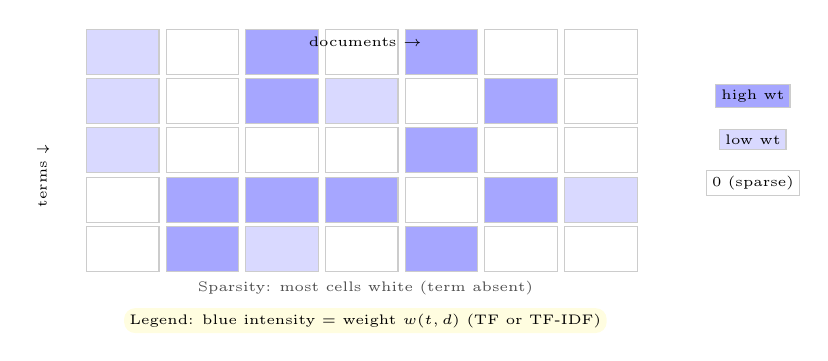
\begin{tikzpicture}[font=\scriptsize, scale=0.92]
  \foreach \r in {0,...,4} \foreach \c in {0,...,6} {
    \pgfmathsetmacro{\v}{int(10*rnd)}
    \ifnum\v<3 \def\cc{blue!35} \else \ifnum\v<5 \def\cc{blue!15} \else \def\cc{white} \fi \fi
    \fill[\cc, draw=gray!40] (1.1*\c, -0.68*\r) rectangle ++(1.0,0.62);
  }
  \node[rotate=90, font=\tiny] at (-0.6,-1.4) {terms $\downarrow$};
  \node[font=\tiny] at (3.85,0.45) {documents $\to$};
  \node[font=\tiny, fill=blue!35, draw=gray!40, inner sep=2pt] at (9.2,-0.3) {high wt};
  \node[font=\tiny, fill=blue!15, draw=gray!40, inner sep=2pt] at (9.2,-0.9) {low wt};
  \node[font=\tiny, fill=white, draw=gray!40, inner sep=2pt] at (9.2,-1.5) {0 (sparse)};
  \node[font=\tiny, text=gray!60!black] at (3.85,-2.95) {Sparsity: most cells white (term absent)};
  \node[font=\tiny, fill=yellow!12, rounded corners, inner sep=2pt] at (3.85,-3.40) {Legend: blue intensity = weight $w(t,d)$ (TF or TF-IDF)};
\end{tikzpicture}
\caption{Term-document matrix heatmap: columns are doc vectors; mostly zeros.}
\label{fig:term-doc}
\end{figure}

\begin{lstlisting}[language=Python, caption={Boolean sets and cosine ranking on the same tiny collection.}, label={lst:boolean-cosine}]
import numpy as np

# Boolean: postings as sets
P_cats = {1,2,4}
P_dogs = {1,3,4}
print("AND:", P_cats & P_dogs)  # {1,4}
print("OR:",  P_cats | P_dogs)  # {1,2,3,4}

# Vector space: raw TF vectors, vocab [cats, dogs]
q  = np.array([1.,1.])
d1 = np.array([1.,1.])   # both
d2 = np.array([3.,0.])   # cats cats cats
d3 = np.array([0.,1.])   # dogs
def cosine(a,b):
    return a.dot(b) / (np.linalg.norm(a)*np.linalg.norm(b))
for name, d in [("d1",d1),("d2",d2),("d3",d3)]:
    print(name, round(cosine(q,d),3))
# d1 1.0 > d2 0.707 > d3 0.707 -> tie broken by other signals
\end{lstlisting}

% ============================================================
\section{Boolean vs.\ Ranked: When Each Wins}\label{sec:compare}
Boolean shines for \emph{exact} needs: ``find docs containing \texttt{SC4021} AND \texttt{PageRank}" as a filter, legal discovery, or when combined with ranking (Boolean filter then rank). Ranked (vector) shines for \emph{best-match} where gradations matter. Modern systems hybridise: use Boolean/phrase for candidate generation, then vector scoring for ranking.

\begin{lstlisting}[language=Python, caption={Hybrid: Boolean filter then cosine re-rank.}, label={lst:hybrid}]
# Hybrid: first Boolean AND, then rank survivors by cosine
docs = {"d1": np.array([1.,1.]), "d2": np.array([3.,0.]), "d3": np.array([0.,1.]), "d4": np.array([1.,0.])}
q = np.array([1.,1.])
candidates = [d for d, v in docs.items() if v[0]>0 and v[1]>0]  # AND cats AND dogs
print("candidates:", candidates)
ranked = sorted(candidates, key=lambda d: cosine(q, docs[d]), reverse=True)
print("ranked:", ranked)
\end{lstlisting}

% ============================================================

% ============================================================
\section{Weighting Preview and Normalization Justification}\label{sec:weight-preview}
\paragraph{Intuition.} The vector example used raw counts. But should ``the'' with count 50 in a long doc outweigh ``PageRank'' with count 2 in a short focused doc? No. Without weighting and length normalization, long docs and frequent words dominate cosine. Ch.~3 will fix this with TF damping and IDF.

\paragraph{Formal tie-in.} Let $\vec{d}_{raw}$ be raw-count vector. Define normalized weighted vector $\vec{d}_{w}=D^{-1}W\vec{d}_{raw}$ where $W$ is diagonal with $idf_t$ and $D$ is length normalizer ($\|\vec{d}\|_2$ or pivoted). Then $\cos(\vec{q}_w,\vec{d}_w)=\vec{q}_w\cdot\vec{d}_w/(\|\vec{q}_w\|\|\vec{d}_w\|)$ already includes $D$, but additional normalizers (double-norm TF, pivoted) further correct for verbosity vs.\ scope: a long doc may be verbose (same topic repeated) or multi-topic (many topics, query covers one) -- the correction differs.

\begin{remark}[Boolean as extremal vector]
Boolean retrieval can be seen as vector retrieval with binary weights and $threshold=1$ for AND, $>0$ for OR, and no normalization. Ranked retrieval generalises it by allowing graded weights and soft thresholds -- one reason industry keeps both layers (Boolean \emph{filters} + vector \emph{rankers}).
\end{remark}

\section{Chapter Notes}
Boolean retrieval powered early systems (STAIRS, Westlaw). Vector space (Salton, 1970s SMART system) introduced geometry to IR. The cosine remains the workhorse even inside neural models (dot products between embeddings are its descendant). Positional and fielded Boolean (title vs.\ body) are handled via extended postings (Ch.~4).

% ============================================================
\section{Exercises}
\begin{enumerate}[label=E2.\arabic*, leftmargin=*, itemsep=0.6em]
  \item \textbf{Boolean sets.} Given $P(a)=\{1,2,3,5\}$, $P(b)=\{2,3,4\}$, $P(c)=\{3,5,6\}$, compute (a) $a$ AND $b$, (b) $a$ OR $b$, (c) $(a$ OR $b)$ AND NOT $c$, (d) $a$ AND $b$ AND $c$. Show sorted postings merges.
  \item \textbf{Cosine by hand.} Vocab \{IR, retrieval, database\}. $\vec{q}=(1,1,0)$, $\vec{d_1}=(2,1,0)$, $\vec{d_2}=(1,0,1)$, $\vec{d_3}=(1,1,1)$. Compute all three cosines, rank, and explain why $d_2$ is penalised.
  \item \textbf{Length normalization.} Doc $A$ has vector $(10,0)$, doc $B$ has $(1,1)$, query $(1,1)$. Euclidean distance ranks $A$ closer to $q$ than $B$ under some centerings; cosine does not. Compute both and explain which better captures topical relevance.
  \item \textbf{Phrase via sets.} How would you support query \texttt{"cats dogs"} (adjacent) using positional postings? Sketch two postings lists with positions and describe the merge that checks adjacency.
  \item \textbf{Hybrid design.} Your system must support ``must contain SC4021 and rank by similarity to \emph{neural IR}.'' Design a two-stage pipeline (filter then rank) and state complexity per stage using postings sizes.
\end{enumerate}

